%!TEX root = ../dokumentation.tex

\chapter{Konzeption}

\section{Separierung von SOS-Klauseln und Nicht-SOS-Klauseln}

PyRes erzeugt bei jeder Beweisprozedur ein Objekt der Klasse ProofState (Beweiszustand). Innerhalb dieses Objekts sind die verarbeiteten und unverarbeiteten Klauseln als zwei Klauselmengen gespeichert. Um SOS-Strategien implementieren zu können, müssen Klauseln des SOS und Klauseln, die nicht zum SOS gehören, unterscheidbar gemacht werden, um sie unterschiedlich behandeln zu können. Dafür werden zwei Konzepte in Betracht gezogen.
\begin{enumerate}
	\item Anstatt den bisher zwei Klauselmengen für verarbeitete und unverarbeitete Klauseln, werden drei Klauselmengen eingesetzt. Jeweils eine Klauselmenge enthält die verarbeiteten Klauseln, die unverarbeiteten SOS-Klauseln und die unverarbeiteten Nicht-SOS-Klauseln.
	\item Jede Klausel erhält eine Zusatzinformation in Form eines Wahrheitswertes, der aussagt, ob sich eine Klausel im SOS befindet oder nicht. Der Wahrheitswert ist als Markierung der Klausel zu verstehen. Das ProofState-Objekt speichert SOS-Klauseln und Nicht-SOS-Klauseln gemischt innerhalb der verarbeiteten und unverarbeiteten Klauselmengen ab.
\end{enumerate}
Beide Lösungsansätze haben Vor- und Nachteile. Ein Vorteil der ersten Variante ist, dass die Klauseln auf Programmebene getrennt voneinander sind. Durch diese Abkapselung könnte es später einfacher und schneller sein, eine neue SOS-Klausel auszuwählen. Diese Variante ist auch einfacher zu verstehen und intuitiver, da die zwei separaten Klauselmengen der theoretischen Grundlage zweier getrennter Mengen entspricht. Ein Nachteil ist, dass der Beweismechanismus stark angepasst werden muss. Zum Beispiel muss für die Resolution eine SOS-Klausel nicht mehr nur mit den verarbeiteten Klauseln kombiniert werden, sondern auch mit den Nicht-SOS-Klauseln. In Hinblick auf die weitere Umsetzung wird es vermutlich Sonderfälle geben, bei denen Nicht-SOS-Klauseln verarbeitet werden müssen. Für die Implementierung solcher Sonderfälle sind zwei getrennte Klauselmengen eher eine Hürde, da die Kombination verschiedener Klauseln komplexer wird. Ein weiterer Nachteil der ersten Variante ist, dass die Information, ob eine Klausel im SOS ist, nicht direkt an die Klausel gebunden ist. Eine Funktion, die eine Klausel übergeben bekommt, kann somit nicht prüfen, ob die übergebene Klausel im SOS ist. Der Funktion müsste deshalb ein zusätzlicher Wahrheitswert übergeben werden, was zu größeren Anpassungen führt.
Für die Implementierung wurde sich nach Abwägung der Vor- und Nachteile für Variante 2 entschieden. Das Hauptargument ist, dass der Code weniger stark angepasst werden muss, aber trotzdem eine einfache Unterscheidungsmöglichkeit eingeführt wird.

\section{Markierung der Klauseln}
Für die Markierung der Klauseln ist eine Funktion vorgesehen, die eine Klauselmenge als Argument übergebene bekommt. Die Funktion soll für jede Klausel den Wahrheitswert für das Set-Of-Support auf wahr oder falsch setzen. Je nachdem, welche SOS-Strategie angewandt wird, wird eine andere Funktion aufgerufen. Für eine bessere Codestruktur ist es sinnvoll, die Funktion in einer Klasse zu kapseln. Für die unterschiedlichen Strategien bietet sich das Konzept der Vererbung an. Es gibt eine abstrakte Oberklasse SosStrategy, die die Methode zur Markierung der Klauselmenge besitzt. Alle davon abgeleiteten Klassen implementieren diese Methode. (siehe Abbildung \ref{fig:sosstrategy0})

Das Programm sollte noch vor Beginn der Beweissuche eine Instanz einer SOS-Klasse erstellen. Welche der Klassen instanziiert wird, soll von einer Eingabeoption des Benutzers abhängig gemacht werden. Die erstellte Instanz soll danach gespeichert werden, damit sie während des Beweisprozesses aufgerufen werden kann. Hierbei wird das Konzept der Polymorphie eingesetzt. Die Beweisprozedur prüft nicht, von welchem Typ das SOS-Objekt ist und weiß somit nicht, welche SOS-Strategie angewandt wird. Dennoch können während der Beweisprozedur die Methoden des SOS-Objekts aufgerufen werden, wodurch die Beweissuche an die SOS-Strategie angepasst wird.

\begin{figure}
	\centering
	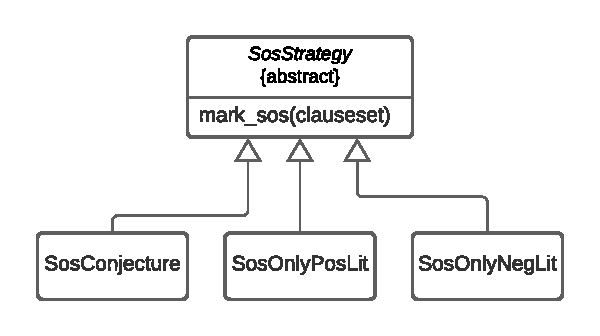
\includegraphics[width=0.7\linewidth]{images/Lucid/SosStrategy0}
	\caption{Klassendiagramm der SOS-Klassen}
	\label{fig:sosstrategy0}
\end{figure}



\section{Anpassung der Beweisprozedur}
\paragraph{bisherige Beweisprozedur}
\begin{figure}
	\centering
	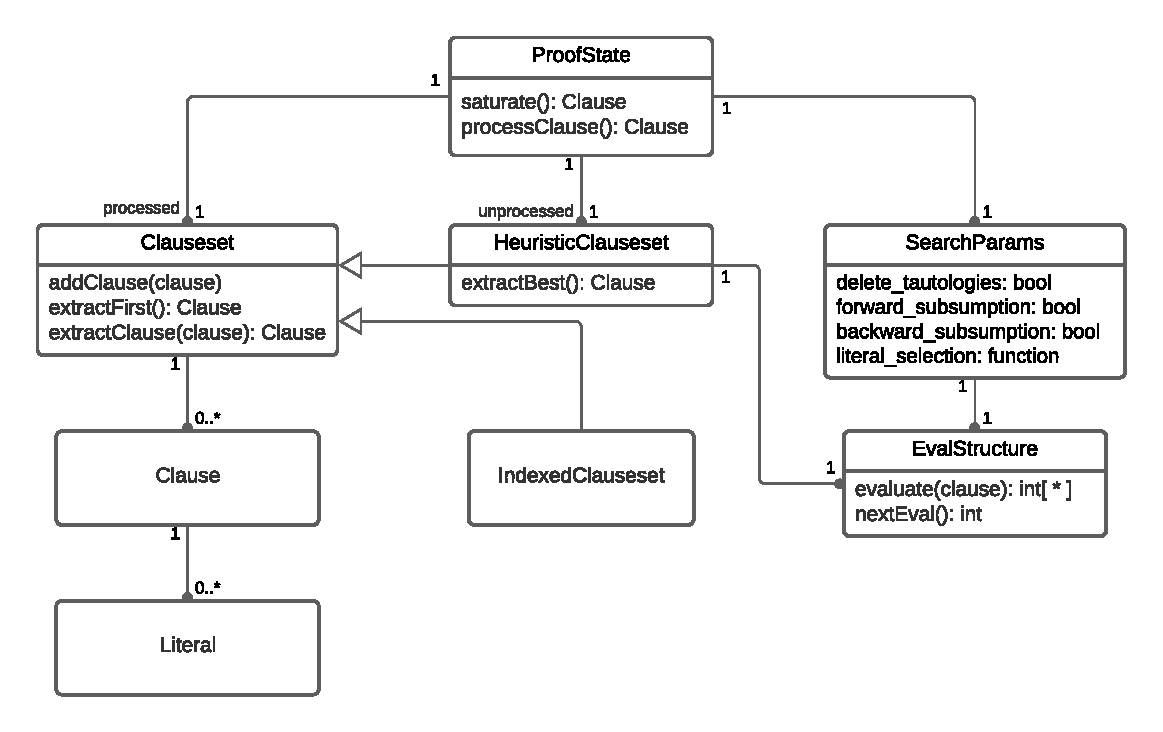
\includegraphics[width=1\linewidth]{images/Lucid/PyResProofState}
	\caption{Klassendiagramm der bisherigen Beweisprozedur}
	\label{fig:pyresproofstate}
\end{figure}

Mit der Beweisprozedur ist die Durchführung des Resolutionsverfahrens gemeint. Die wird begonnen, nachdem das Einlesen der Datei und die Initialisierung der Klauseln abgeschlossen ist. PyRes startet die Prozedur, indem die Methode saturate() der ProofState-Instanz aufgerufen wird.

Das Proofstate-Objekt hält Referenzen zu drei Objekten (siehe Abbildung \ref{fig:pyresproofstate})
\begin{enumerate}
	\item Eine Instanz der Klasse SearchParams. Es handelt sich dabei um einen Container, der speichert, welche Beweis-Optimierungen durchgeführt werden, zum Beispiel ob Tautologien gelöscht werden sollen.
	\item Eine Klauselmenge mit allen unverarbeiteten Klauseln. Diese Menge ist von der Klasse "`HeuristicClauseset"', welche von der gewöhnlichen Klauselmenge "`Clauseset"' erbt. Die Klasse Clauseset implementiert einige einfache Methoden zur Verwaltung von Klauseln (z.B. hinzufügen, entfernen). HeuristicClauseset hat zusätzlich die Methode extractBest(), welche die geeignetste Klausel auswählt. Wie geeignet eine Klausel ist, wird von den gewählten Heuristiken bestimmt, die in der Klasse EvalStructure gekapselt sind.
	\item Eine Klauselmenge mit verarbeiteten Klauseln. Diese Klauselmenge ist entweder von der Klasse Clauseset oder der vererbten Klasse IndexedClauseset. Welche der beiden Klassen verwendet wird, hängt davon ab, ob das Indexing als Optimierung aktiviert ist. Für die SOS-Implementierung hat das Indexing keine weitere Bedeutung.
\end{enumerate}

\begin{figure}
	\centering
	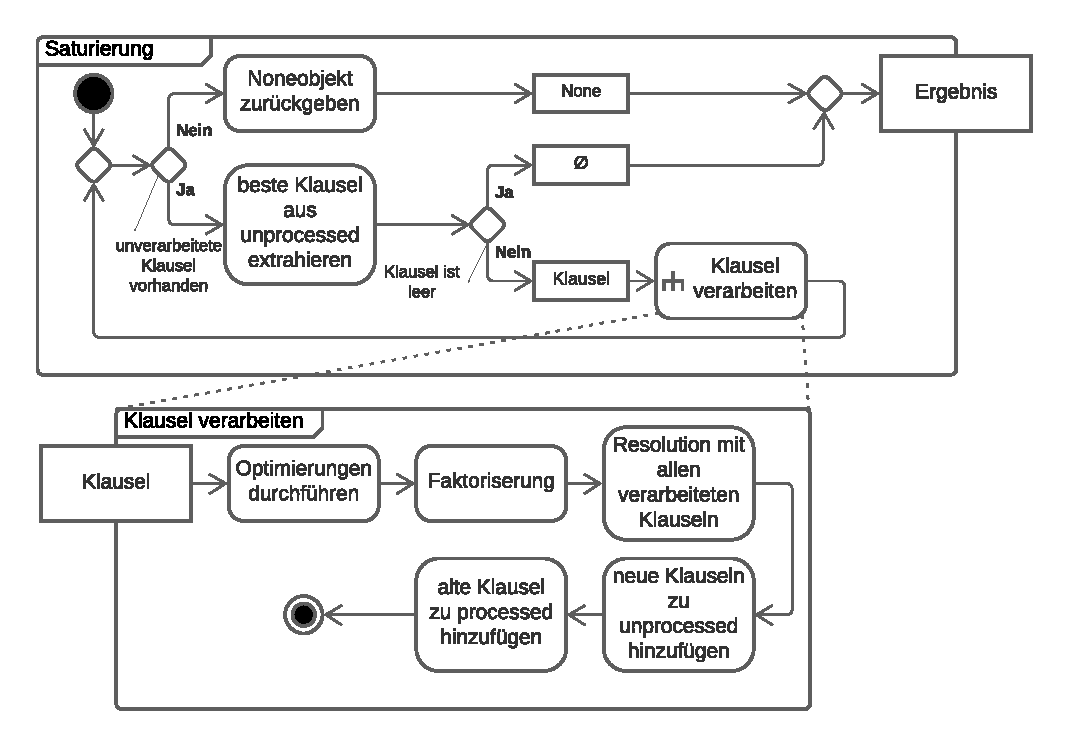
\includegraphics[width=1\linewidth]{images/Lucid/ActivityProof}
	\caption{Aktivitätsdiagramm der Beweisprozedur}
	\label{fig:activityproof}
\end{figure}


Der Algorithmus, den die saturate()-Methode durchführt, ist im Aktivitätsdiagramm in Abbildung \ref{fig:activityproof} dargestellt. Zusammengefasst werden Klauseln solange durch Faktorisierung und Resolution mit den bereits verarbeiteten Klauseln abgearbeitet, bis entweder der leere Klausel gefunden wurde, oder keine Klauseln mehr übrig sind.
Im ersten Fall wird die leere Klausel zurückgegeben, im zweiten Fall None. Das Schlüsselwort None repräsentiert in Python ein undefiniertes Objekt und ist vergleichbar mit einem null-Pointer in der Sprache C.

\paragraph{SOS-Konzept 1: Nicht-SOS zu processed hinzufügen}

Eine sehr simple Art, die SOS-Strategien umzusetzen, ist, alle Nicht-SOS-Klauseln als verarbeitet anzusehen. Das Programm soll vor der Ausführung der Beweisprozedur alle SOS-Klauseln markieren. Die saturate()-Methode entfernt dann alle Nicht-SOS-Klauseln aus der unverarbeiteten Klauselmenge und fügt sie zur Menge der verarbeiteten Klauseln hinzu. Der Auswahlalgorithmus, der die nächstbeste Klausel aus den unverarbeiteten extrahiert, wird garantiert eine SOS-Klausel auswählen, da in der Klauselmenge nur SOS-Klauseln enthalten sind. Resolution zweier Nicht-SOS-Klauseln ist somit nicht möglich. Resolution einer SOS-Klausel mit einer Nicht-SOS-Klausel ist weiterhin erlaubt, denn die ausgewählte SOS-Klausel kann mit den (verarbeiteten) Nicht-SOS-Klauseln kombiniert werden. 

Die SOS-Strategien sind in Kombination mit den Optimierungsstrategien Literalselektion und geordneter Resolution nicht vollständig (Quelle). Grund dafür ist, dass der gesuchte Beweis die Resolution zweier Nicht-SOS-Klauseln erfordern könnte. Wird SOS-Konzept 1 zur Beweissuche eingesetzt, muss darauf geachtet werden, dass die anderen beiden Optimierungen deaktiviert sind. Andernfalls kann es passieren, dass ein unerfüllbares Problem als erfüllbar eingestuft wird. 

\paragraph{SOS-Konzept 2: SOS und Nicht-SOS mit unterschiedlicher Priorität verarbeiten}

Ziel ist, eine SOS-Implementierung zu schaffen, die kompatibel mit Literalselektion und geordneter Resolution ist. Somit darf die Resolution zweier Nicht-SOS-Klauseln nicht komplett verboten werden, sondern muss weiterhin stattfinden. Das Konzept sieht vor, SOS-Klauseln mit einer höheren Priorität abzuarbeiten als Nicht-SOS-Klauseln. Dazu wird ein konstantes Verhältnis $r$ eingeführt, das vorgibt, wie viele SOS-Klauseln verarbeitet werden, bevor die nächste Nicht-SOS-Klausel verarbeitet wird. Ein Verhältnis von 3 würde bedeutet, dass immer 3 SOS-Klauseln verarbeitet werden und danach eine Nicht-SOS-Klausel.

Wenn als nächstes eine SOS-Klausel an der Reihe wäre, aber es keine unverarbeitete mehr gibt, dann wird stattdessen die nächstbeste Nicht-SOS-Klausel ausgesucht. Das gleiche gilt, wenn es keine unverarbeiteten Nicht-SOS-Klauseln mehr gibt. PyRes soll ein Problem erst dann als erfüllbar einstufen, wenn es weder SOS- noch Nicht-SOS-Klauseln mehr gibt, also die Menge der unverarbeiteten Klauseln leer ist.


Egal, wie groß das gewählte Verhältnis $r$ ist, die Beweissuche wird immer vollständig bleiben. Das liegt daran, dass jede Nicht-SOS-Klausel für beliebiges $r$ in endlicher Zeit abgearbeitet wird. Somit kann es nicht passieren, dass einzelne Klauseln während des Beweisprozesses nicht berücksichtigt werden und die Beweisfindung verhindern.
Ein unendlicher großer Wert für $r$ würde bedeuten, dass Nicht-SOS-Klauseln erst dann ausgewählt werden, wenn es keine SOS-Klauseln mehr gibt. Wenn dieser Fall eintritt, dann und genau dann ist die Erfüllbarkeit des SOS gezeigt. Es kann passieren, dass das SOS erfüllbar ist und diese Erfüllbarkeit nicht nachgewiesen werden kann, da unendlich viele Klauseln abgeleitet werden können. In diesem Fall werden nie Nicht-SOS-Klauseln ausgewählt, wodurch die leere Menge nie hergeleitet werden kann. 

Zusammenfassend gilt: Damit die Vollständigkeit erhalten bleibt, kann für $r$ jede positive ganze Zahl gewählt werden. Es ist davon auszugehen, dass sehr große Werte und sehr kleine Werte die Effizienz der Strategie reduzieren und es ein Optimum in der Mitte gibt. Für große Werte werden Nicht-SOS-Klauseln kaum verarbeitet, wodurch die Unerfüllbarkeit erst spät nachweisbar wird. Für kleine Werte ist anzunehmen, dass der potenzielle Vorteil der SOS-Strategie verloren geht.
